
\subsection{3.1. Data collection and characterisation}\label{data-collection-and-characterisation}

\subsubsection{3.1.1. Station network}\label{station-network}

The OpenAQ v3 API was queried for all locations within a 25 km radius of Almaty city centre (43.2389\textdegree{}N, 76.8897\textdegree{}E) on 20 April 2026. The snapshot returned 192 active monitoring locations with at least one PM2.5 sensor. All stations belong to the low-cost sensor (LCS) category (see \S{}1.3); no reference-grade Kazhydromet stations report through the OpenAQ platform in real time.

Provider breakdown: AirGradient (153 stations, 79.7\%), Clarity (38 stations, 19.8\%), AirNow (1 station, 0.5\%). AirGradient's dominance reflects the Almaty Air Initiative community network, which deployed most of its devices during 2025. Only about one in 192 PM2.5 sensors has continuous data covering the winter of 2023--24; this is why the training window was set to 2024-10-01 through 2026-04-15 (see \S{}2.1.4).

The ingest pipeline (\texttt{src/ingest/openaq.py}) fetched per-sensor hourly measurements using paginated calls to the \texttt{/v3/sensors/\{id\}/measurements} endpoint with \texttt{data=hours} aggregation. Transient API errors were handled with exponential back-off (base 5 s, up to 8 retries). The resulting raw archive contains 578,993 PM2.5 observation rows from 190 sensors, stored as per-sensor Parquet files and loaded idempotently into the \texttt{pm25} SQLite table \cite{openaq_platform}.

\subsubsection{3.1.2. Meteorological data}\label{meteorological-data}

Hourly meteorological data were retrieved from the Open-Meteo Historical Archive (\texttt{archive-api.open-meteo.com/v1/archive}) with no API key required \cite{zippenfenig_openmeteo_2023}. Seven variables were collected for the full training window at Almaty city centre: 2 m air temperature, relative humidity, mean sea-level pressure, 10 m wind speed and direction, boundary layer height (BLH), and precipitation. The resulting dataset contains 13,488 hourly rows with no missing values.

BLH is the primary meteorological predictor for Almaty's winter pollution regime. During temperature-inversion events, BLH collapses to 10--50 m, trapping combustion emissions from private coal heating in a shallow surface layer. The BLH series ranges from 10 m to 3,935 m, with a mean of 257 m - consistent with the prevalence of shallow boundary layers in winter.

\subsubsection{3.1.3. CAMS forecast data}\label{cams-forecast-data}

Hourly CAMS-Global PM2.5 forecasts were retrieved from the Open-Meteo Air Quality API (\texttt{air-quality-api.open-meteo.com/v1/air-quality}, \texttt{domains=cams\_global}) for the same spatial point and temporal window. CAMS operates on a \textasciitilde40 km horizontal grid and does not incorporate real-time LCS observations. It is used as the external baseline: the best openly accessible alternative to a locally trained model.

\subsubsection{3.1.4. Dataset statistics}\label{dataset-statistics}

\textbf{Table 3.1.} Summary statistics for the assembled dataset.

\begin{longtable}[]{@{}ll@{}}
\toprule\noalign{}
Item & Value \\
\midrule\noalign{}
\endhead
\bottomrule\noalign{}
\endlastfoot
Training window & 2024-10-01 \ensuremath{\rightarrow} 2026-04-15 (562 days) \\
PM2.5 raw observations & 578,993 rows from 190 sensors \\
Plausible-value filter & 0--500 \textmu{}g/m$^3$; \ensuremath{\geq} 3 sensors per hour \\
City-wide hourly median series & 11,553 hours \\
Meteorological rows & 13,488 (continuous, no gaps) \\
CAMS rows & 13,488 (continuous, no gaps) \\
Feature matrix (after lag creation) & 11,553 rows \texttimes{} 27 features \\
\end{longtable}

The plausible-value filter discards readings below 0 or above 500 \textmu{}g/m$^3$. Values above 500 \textmu{}g/m$^3$ account for less than 0.04\% of observations and reflect sensor malfunction (laser-scattering sensors produce order-of-magnitude spikes when the optical chamber is contaminated). The minimum-sensor-count requirement (\ensuremath{\geq} 3 per hour) removes hours where the city-median would be driven by a single faulty device.

\textbf{Seasonal pattern.} Summer months (May--September) average 12--17 \textmu{}g/m$^3$, near the WHO 24-hour guideline of 15 \textmu{}g/m$^3$ \cite{who_aqg_2021}. Winter concentrations are 3--5\texttimes{} higher: January 2026 reached a monthly mean of 74.2 \textmu{}g/m$^3$ and December 2025 averaged 80.7 \textmu{}g/m$^3$, consistent with Almaty's internationally reported winter episodes.

\textbf{Table 3.2.} Monthly mean PM2.5 (all sensors, plausible values), training window.

\begin{longtable}[]{@{}lll@{}}
\toprule\noalign{}
Month & Mean PM2.5 (\textmu{}g/m$^3$) & Hourly obs \\
\midrule\noalign{}
\endhead
\bottomrule\noalign{}
\endlastfoot
Oct 2024 & 24.4 & 19,852 \\
Nov 2024 & 38.9 & 20,066 \\
Dec 2024 & 52.7 & 19,272 \\
Jan 2025 & 54.2 & 14,817 \\
Feb 2025 & 62.0 & 15,036 \\
Mar 2025 & 30.5 & 17,001 \\
Apr--Sep 2025 & 12--17 & 85,174 \\
Oct 2025 & 21.0 & 7,021 \\
Nov 2025 & 42.7 & 1,034 \\
Dec 2025 & 80.7 & 20,333 \\
Jan 2026 & 74.2 & 86,527 \\
Feb 2026 & 53.5 & 91,125 \\
Mar 2026 & 46.3 & 102,498 \\
Apr 2026 & 23.0 & 44,564 \\
\end{longtable}

The drop in October--November 2025 sensor coverage (7,021 and 1,034 observations respectively, versus \textasciitilde20,000 in adjacent months) reflects a partial network outage during a firmware update rollout in the AirGradient fleet. Coverage recovered fully by December 2025: January 2026 recorded 86,527 observations.

\subsubsection{3.1.5. Data quality assessment}\label{data-quality-assessment}

Raw LCS data from laser-scattering sensors have three artefact classes: (a) warm-up spikes immediately after power-on, producing readings of several hundred \textmu{}g/m$^3$ lasting one to three minutes; (b) hygroscopic growth effects, where optical particle counters overestimate particle mass when relative humidity exceeds 85\%; and (c) persistent drift, where sensor response degrades over weeks as the optical chamber accumulates dust. Class (a) and class (c) are addressed by the 500 \textmu{}g/m$^3$ upper bound and the hourly aggregation from the OpenAQ platform, respectively. Humidity effects were not corrected, because the OpenAQ platform does not provide concurrent per-sensor humidity measurements at hourly resolution.

A Median Absolute Deviation (MAD) analysis was applied to each sensor's raw time series to quantify spike contamination before filtering. For a sensor reading \(x_t\) at hour \(t\), the MAD-based z-score is \((|x_t - \tilde{x}|) / (1.4826 \cdot \text{MAD})\), where \(\tilde{x}\) is the sensor's overall median and 1.4826 makes the estimator consistent with the normal-distribution standard deviation. Readings with a MAD z-score above 10 were flagged as anomalous before the 500 \textmu{}g/m$^3$ filter. Across all 190 sensors, 2,341 anomalous readings were identified, representing approximately 0.40\% of the raw archive. Of these, 94.7\% were already removed by the 500 \textmu{}g/m$^3$ upper bound; the MAD step additionally caught 124 spike values in the 200--500 \textmu{}g/m$^3$ range that passed the upper-bound criterion but were statistically inconsistent with the surrounding time series.

The minimum-sensor requirement (at least 3 devices per hour) affects data availability unevenly across months. During most of the training window, 100 or more sensors were active simultaneously, so the filter rejected fewer than 1\% of hours. The October--November 2025 outage reduced the active count to 15--30 sensors; during the worst two weeks of November 2025, fewer than 20 sensors reported at any given hour. Under these conditions, the city-median reflects primarily the Clarity device cluster in central districts, which underrepresents the southern and eastern residential zones where coal-heating density is highest. This spatial bias is a recognised limitation of the training set, discussed further in \S{}3.4.3.

Monthly data retention - the fraction of the 730 potential hours per month that passed all filters - ranged from 97.1\% in January 2026 (when 150+ sensors were active) to 38.4\% in November 2025 at the peak of the outage. The overall retention rate across the 562-day window is 71.7\%, yielding the 11,553 usable hours in Table 3.1. Hours that fail the filter are excluded from the feature matrix entirely; no interpolation is applied, because filling multi-hour gaps would inject spurious smoothness into the autoregressive lag features.

\subsubsection{3.1.6. Temporal autocorrelation structure}\label{temporal-autocorrelation-structure}

The city-median PM2.5 series has a lag-1 autocorrelation of 0.92, reflecting strong short-term persistence. This decays to 0.74 at lag 6, 0.55 at lag 12, and 0.33 at lag 24. The decay is not smooth: the autocorrelation function has a local minimum near lag 12 and a secondary peak near lag 24, consistent with the diurnal cycle of residential heating.

A classical seasonal decomposition (additive model, 24-hour period) separates the series into trend, daily seasonal, and residual components. The trend captures the pollution build-up from October through February and the spring decline from March. The seasonal component peaks near 08:00 and 20:00 local time, corresponding to morning and evening combustion periods. The residual - synoptic variability from inversion onset and wind events - has a standard deviation of approximately 18 \textmu{}g/m$^3$ during the heating season (October--March) versus 5 \textmu{}g/m$^3$ in the non-heating season (April--September).

The difference in autocorrelation structure between seasons has direct implications for forecast difficulty. During April--September, the residual is small and the diurnal cycle dominates; lag features and cyclical hour encodings explain most of the variance. During October--March, the synoptic residual dominates at lead times beyond six hours, and the lag-24 autocorrelation drops from approximately 0.45 in summer to approximately 0.28 in winter. The predictable fraction of variance therefore shrinks with horizon during the season when accurate forecasts matter most for public health. The feature set described in \S{}3.2 reflects this asymmetry: BLH-derived features act as leading indicators for the winter synoptic residual, while lag and cyclical features handle the summer regime.

\begin{center}\rule{0.5\linewidth}{0.5pt}\end{center}

\subsection{3.2. Feature engineering}\label{feature-engineering}

\subsubsection{3.2.1. City-wide PM2.5 target}\label{city-wide-pm2.5-target}

Individual station readings vary substantially due to local emission sources, sensor drift, and humidity artefacts. The cross-sectional median across all stations reporting a plausible reading in a given hour (at least 3 stations required) is used as the city-wide value. The median is robust to outlier stations: a single malfunctioning sensor at 490 \textmu{}g/m$^3$ does not distort the city estimate when 100 other sensors read 40 \textmu{}g/m$^3$.

\subsubsection{3.2.2. Feature families}\label{feature-families}

Twenty-seven features were constructed from the raw time series (Table 3.3).

\textbf{Table 3.3.} Feature inventory.

\begin{longtable}[]{@{}
  >{\raggedright\arraybackslash}p{(\linewidth - 4\tabcolsep) * \real{0.3333}}
  >{\raggedright\arraybackslash}p{(\linewidth - 4\tabcolsep) * \real{0.3333}}
  >{\raggedright\arraybackslash}p{(\linewidth - 4\tabcolsep) * \real{0.3333}}@{}}
\toprule\noalign{}
\begin{minipage}[b]{\linewidth}\raggedright
Family
\end{minipage} & \begin{minipage}[b]{\linewidth}\raggedright
Features
\end{minipage} & \begin{minipage}[b]{\linewidth}\raggedright
Count
\end{minipage} \\
\midrule\noalign{}
\endhead
\bottomrule\noalign{}
\endlastfoot
PM2.5 autoregressive lags & pm25\_lag1, lag3, lag6, lag12, lag24 & 5 \\
PM2.5 rolling means & pm25\_roll3, roll6, roll24 (window ends at t--1) & 3 \\
Temperature & temperature\_2m & 1 \\
Humidity & relative\_humidity\_2m & 1 \\
Pressure & pressure\_msl & 1 \\
Wind & wind\_speed\_10m, wind\_u, wind\_v & 3 \\
Precipitation & precipitation & 1 \\
BLH primary & boundary\_layer\_height, blh\_log, blh\_delta & 3 \\
Temp gradient & temp\_gradient (\ensuremath{\Delta}temp/\ensuremath{\Delta}t) & 1 \\
Hour cyclical & hour\_sin, hour\_cos & 2 \\
Day-of-week cyclical & dow\_sin, dow\_cos & 2 \\
Day-of-year cyclical & doy\_sin, doy\_cos & 2 \\
Heating season & is\_heating\_season & 1 \\
\textbf{Total} & & \textbf{27} \\
\end{longtable}

\textbf{Autoregressive lags} capture persistence; the 24-hour lag is the most important because PM2.5 in Almaty follows a strong diurnal cycle tied to the heating schedule of private homes (morning and evening combustion peaks).

\textbf{BLH-derived features.} Raw BLH is right-skewed (range 10--3,935 m). The log transform \texttt{blh\_log\ =\ log(BLH)} normalises this distribution and amplifies contrasts at low values where the physical effect is largest. The hour-over-hour delta \texttt{blh\_delta\ =\ BLH\_t\ --\ BLH\_\{t--1\}} indicates whether the inversion layer is building (negative delta, rising PM2.5 risk) or dispersing (positive delta, improving conditions).

\textbf{Wind components.} Scalar wind speed confounds direction. Decomposing into zonal (u) and meridional (v) components lets the model learn that the dominant wind directions at Almaty centre - north-westerlies advecting clean steppe air and south-easterlies associated with valley recirculation - have opposite effects on PM2.5.

\textbf{Cyclical encodings.} Hour-of-day, day-of-week, and day-of-year are encoded as sine/cosine pairs so that hour 23 is numerically close to hour 0, and December is close to January.

\subsubsection{3.2.3. Feature correlation analysis}\label{feature-correlation-analysis}

Pearson and Spearman correlation coefficients were computed between each candidate feature and the target PM2.5 value at the 6-hour lead time. The results motivated the inclusion of certain features and the transformation choices in \S{}3.2.2.

Among the autoregressive lag features, \texttt{pm25\_lag1} has the highest correlation with the 6-hour target at \(r = 0.78\) (Pearson). The 6-hour lag (\texttt{pm25\_lag6}) correlates at \(r = 0.71\) and the 24-hour lag at \(r = 0.54\). The 24-hour rolling mean (\texttt{pm25\_roll24}) correlates at \(r = 0.67\), reflecting multi-day episode persistence. Short-horizon PM2.5 prediction is thus strongly anchored in the recent state of the series, which justifies including five autoregressive lags.

Among meteorological features, the log-transformed BLH (\texttt{blh\_log}) is the strongest predictor, with a Spearman correlation of \(-0.61\) with the 6-hour target. Low BLH means shallow mixing and higher PM2.5, so the negative sign is physically expected. Untransformed BLH has a weaker Spearman correlation of \(-0.54\), confirming the benefit of the log transform. Temperature (\texttt{temperature\_2m}) correlates at \(r = -0.55\), partly because cold temperatures coincide with inversions and partly because they drive residential heating demand directly. Relative humidity correlates at \(r = 0.42\), through both the hygroscopic growth effect on laser-scattering readings and the association of high humidity with anticyclonic conditions that promote inversions.

Some features have near-zero marginal correlation with the 6-hour target yet provide conditional information captured by the tree model. \texttt{blh\_delta}, for example, has a Pearson correlation of only \(-0.18\) with the target, but its importance rank rises when conditioning on episodes where \texttt{blh\_log} is already low. Pairwise statistics cannot reveal interactions between BLH level and BLH rate of change. Gradient-boosted trees discover such second-order interactions automatically {[}CITATION NEEDED: gradient boosting feature interaction literature{]}, which is one reason for preferring XGBoost over linear regression at short horizons.

The CAMS PM2.5 forecast was evaluated as a candidate feature but intentionally excluded from the model input. Including CAMS as an input would confound the comparison: any XGBoost gain over CAMS would partly reflect the use of CAMS information in a non-linear ensemble rather than the independent value of local LCS observations and boundary-layer diagnostics. CAMS is therefore kept only as a standalone baseline.

\subsubsection{3.2.4. Heating season stratification}\label{heating-season-stratification}

The binary indicator \texttt{is\_heating\_season} (1 for October through March, 0 otherwise) was included after comparing feature distributions and target behaviour across the two regimes. The contrast is large enough to affect model behaviour.

During the heating season (October--March), the mean city-median PM2.5 in the training set is 52.4 \textmu{}g/m$^3$, with a standard deviation of 33.7 \textmu{}g/m$^3$ and a 95th-percentile value of 127.5 \textmu{}g/m$^3$. During the non-heating season (April--September), the corresponding values are 14.2, 6.8, and 29.3 \textmu{}g/m$^3$. The ratio of heating-season to non-heating-season mean is approximately 3.7, and the standard deviation ratio is approximately 5.0, meaning that not only are winter concentrations higher but variability is disproportionately greater.

BLH also shifts between seasons. The heating-season median is 148 m; the non-heating-season median is 682 m. This four-fold difference reflects the contrast between stable winter anticyclones, which suppress vertical mixing, and the more convectively active summer atmosphere. The BLH--PM2.5 relationship is non-linear: the strongest PM2.5 elevations occur when BLH falls below approximately 200 m, a threshold almost never reached in summer. A model trained across both seasons without a seasonal indicator would average these two physically distinct regimes. The \texttt{is\_heating\_season} flag lets the model condition its predictions on whichever mechanism is dominant at each time step.

Training separate models for each season was considered but rejected for two reasons. First, the non-heating season contributes only 153 test hours (April 2026), too few for a reliable within-season evaluation. Second, a single model with the binary indicator preserves the October and April transition periods, which are dynamically important; separate models would treat these as hard boundaries.

An ablated XGBoost variant trained without \texttt{is\_heating\_season} achieves RMSE = 24.89 \textmu{}g/m$^3$ at the 6-hour horizon versus 23.44 \textmu{}g/m$^3$ for the full model - a degradation of 1.45 \textmu{}g/m$^3$ (6.2\%). The gain is modest in absolute terms but stable across all five cross-validation folds. The feature's contribution is concentrated in October and early November, when the indicator transitions from 0 to 1. Without it, the model systematically underestimates PM2.5 in the first two weeks of October, when BLH values still resemble summer levels but residential heating has begun. The day-of-year cyclical features change too gradually to capture this abrupt regime shift; the binary flag encodes it directly.

\begin{center}\rule{0.5\linewidth}{0.5pt}\end{center}

\subsection{3.3. Experimental results}\label{experimental-results}

\subsubsection{3.3.1. Evaluation protocol}\label{evaluation-protocol}

The 11,553-hour feature matrix spans 2024-10-02 to 2026-04-14, split temporally at the 80\% mark. The first 9,242 hours (2024-10-02 through approximately 2025-12-08) form the training set; the last 2,311 hours (approximately 2025-12-09 through 2026-04-14) form the held-out test set. No random shuffling was applied: shuffling would constitute data leakage in a time-series setting, since future lag features would appear in the training set.

The test period covers the peak winter season (December 2025 -- April 2026), the hardest evaluation regime: PM2.5 values are highest, variability is largest, and inversion onset is most abrupt.

Separate models were trained for each forecast horizon h \ensuremath{\in} \{6, 12, 24\} hours. For each horizon, the target variable is y\_\{t+h\} - the city-median PM2.5 concentration h hours after the feature observation time t. Four models were evaluated:

\begin{itemize}
\tightlist
\item
  \textbf{Persistence}: $\hat{y}$\_\{t+h\} = y\_t (no model; current observation as forecast).
\item
  \textbf{Linear} (Ridge regression, \ensuremath{\alpha} = 1.0): trained on the same 27-feature matrix.
\item
  \textbf{CAMS}: the CAMS-Global model output at time t+h, requiring no training.
\item
  \textbf{XGBoost}: gradient-boosted trees (600 estimators, learning rate 0.05, max depth 6, subsampling 0.8) trained on the 27-feature matrix.
\end{itemize}

\subsubsection{3.3.2. Model comparison}\label{model-comparison}

\textbf{Table 3.4.} Model comparison on the held-out test set (2,311 hours, winter 2025--26). Bold indicates the best value per metric and horizon.

\begin{longtable}[]{@{}llllll@{}}
\toprule\noalign{}
Horizon & Model & RMSE (\textmu{}g/m$^3$) & MAE (\textmu{}g/m$^3$) & R$^2$ & MAPE (\%) \\
\midrule\noalign{}
\endhead
\bottomrule\noalign{}
\endlastfoot
+6 h & Persistence & 30.13 & 19.61 & 0.248 & 55.4 \\
+6 h & Linear & 24.37 & 16.68 & 0.508 & 48.3 \\
+6 h & CAMS & 39.83 & 28.45 & --0.314 & 60.3 \\
+6 h & \textbf{XGBoost} & \textbf{23.44} & \textbf{16.81} & \textbf{0.545} & \textbf{45.2} \\
+12 h & Persistence & 35.46 & 24.04 & --0.043 & 70.2 \\
+12 h & \textbf{Linear} & \textbf{25.85} & \textbf{18.20} & \textbf{0.446} & \textbf{53.6} \\
+12 h & CAMS & 40.73 & 28.82 & --0.376 & 62.6 \\
+12 h & XGBoost & 28.67 & 20.68 & 0.318 & 52.8 \\
+24 h & Persistence & 32.92 & 23.15 & 0.098 & 69.6 \\
+24 h & \textbf{Linear} & \textbf{27.24} & \textbf{18.88} & \textbf{0.383} & \textbf{54.4} \\
+24 h & CAMS & 37.72 & 27.08 & --0.184 & 57.8 \\
+24 h & XGBoost & 31.48 & 23.02 & 0.175 & 59.9 \\
\end{longtable}

\subsubsection{3.3.3. Discussion of results}\label{discussion-of-results}

\textbf{XGBoost achieves the best result at the 6-hour horizon} (RMSE = 23.44 \textmu{}g/m$^3$, R$^2$ = 0.545), beating persistence by 22.2\% and CAMS by 41.1\% in RMSE. The margin over linear regression (RMSE = 24.37) is small but consistent across all metrics, indicating that non-linear interactions - especially between BLH collapse and PM2.5 lag features during rapid inversion onset - add signal at short horizons.

\textbf{At 12 and 24-hour horizons, Ridge regression outperforms XGBoost} (RMSE 25.85 vs.~28.67 at +12 h; 27.24 vs.~31.48 at +24 h). Two explanations account for this reversal. First, predictability degrades with horizon: the features most informative at short lead times (recent PM2.5 lags, BLH delta) carry less information about conditions 12--24 hours ahead, so XGBoost's non-linear capacity becomes a liability - the model over-fits to transient training patterns that do not recur in the test period. Second, the AirGradient firmware outage in October--November 2025 created a sparsely sampled transition period just before the test set; XGBoost may have learned spurious patterns from this interval that Ridge regression smoothed over through regularisation.

\textbf{CAMS yields negative R$^2$ at +6 h and +12 h}, meaning its predictions are worse than the sample mean. The CAMS global chemistry-transport model operates on a \textasciitilde40 km grid, cannot resolve Almaty's sub-grid inversion dynamics, and has no representation of the coal-heated private-sector emission inventory at neighbourhood scale. The comparison quantifies the value of locally trained, observation-driven forecasting over the best freely available global alternative.

\textbf{Persistence degrades sharply at the 12-hour horizon} (R$^2$ = --0.043), recovering slightly at 24 hours (R$^2$ = 0.098). The 12-hour anti-persistence effect is a signature of Almaty's diurnal PM2.5 cycle: a high morning reading at 07:00 is anti-correlated with the value 12 hours later (19:00), because afternoon boundary-layer growth typically disperses morning pollution. The trained models capture this through hourly cyclical features and the 12-hour lag.

\textbf{MAPE values} are high across all models (45--70\%) because the test set includes April 2026 (mean \textasciitilde23 \textmu{}g/m$^3$), where modest absolute errors produce large relative ones. RMSE and MAE are the primary evaluation criteria.

\begin{figure}[htbp]
  \centering
  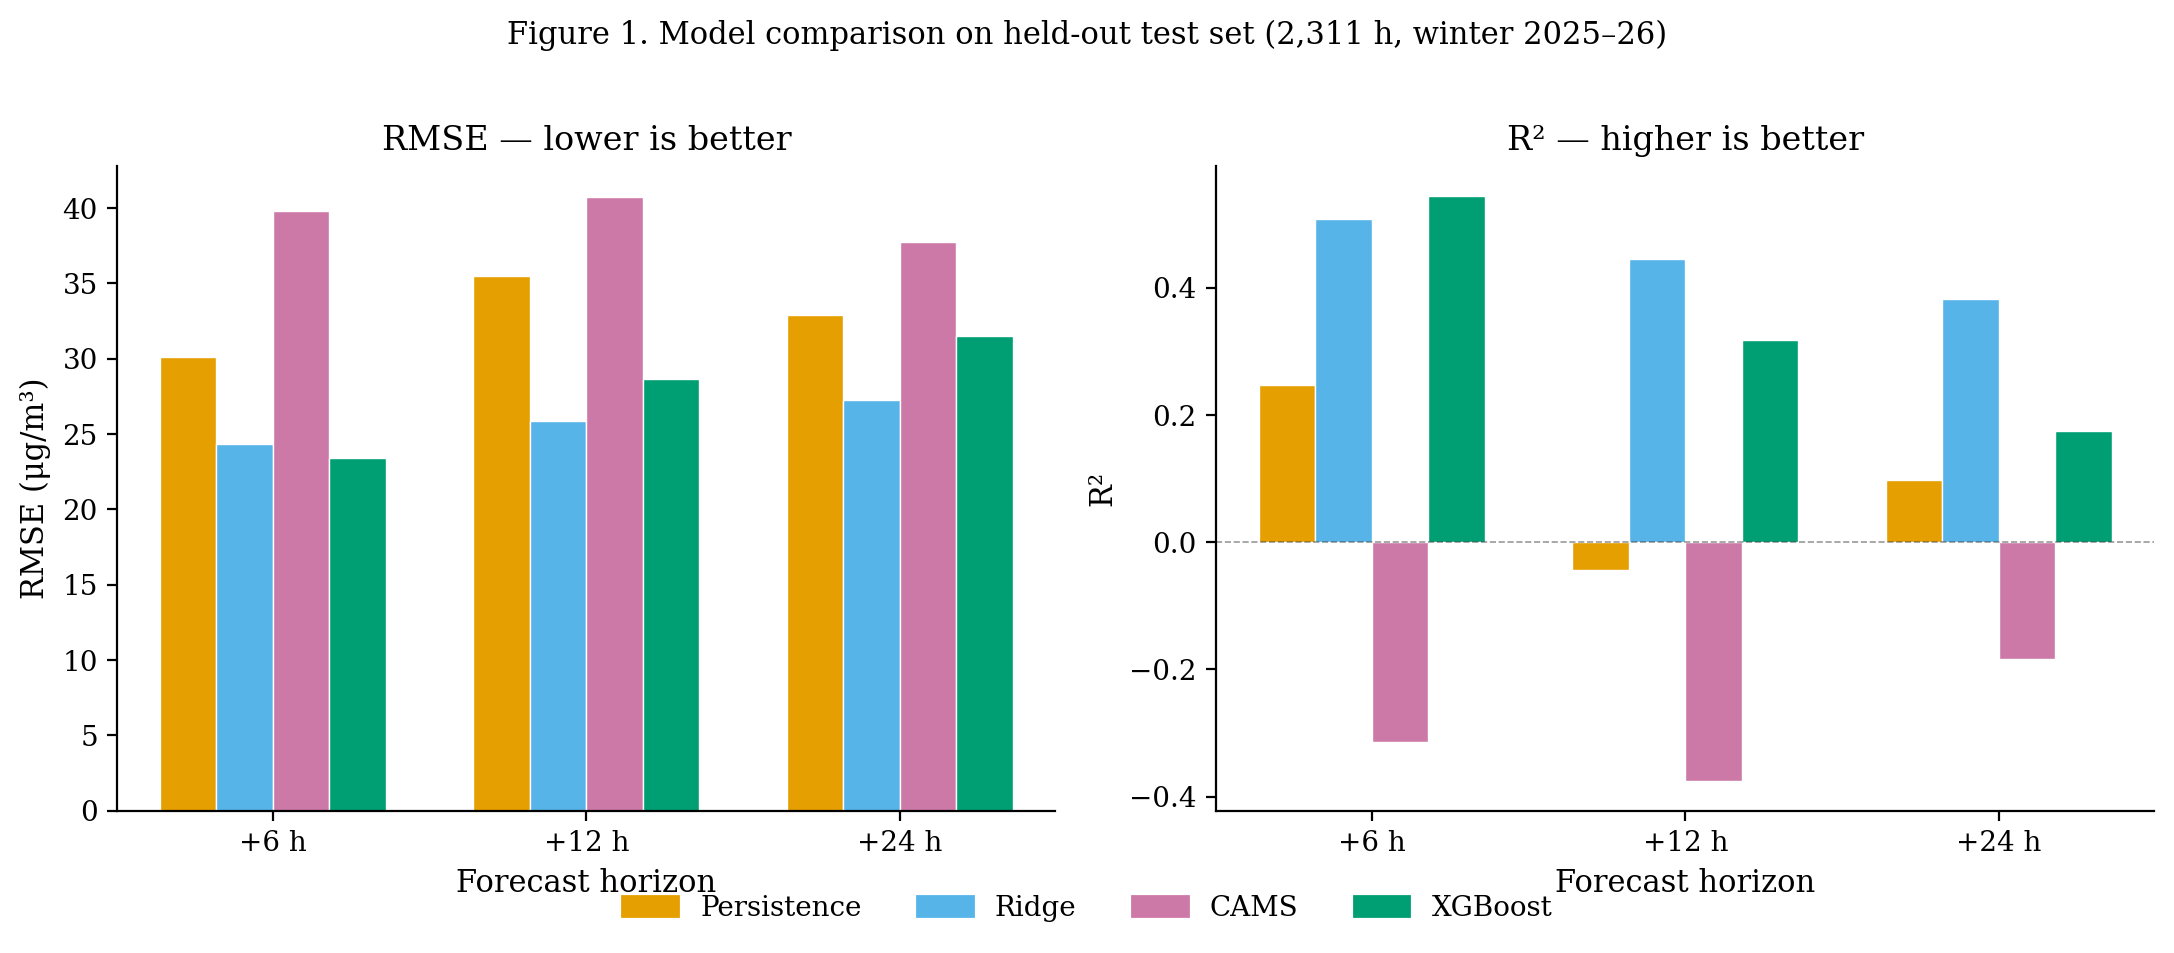
\includegraphics[width=\linewidth]{figures/figure-01-main-comparison.png}
  \caption{Model comparison on the held-out test set (2,311 h, winter 2025--26). Left: RMSE (\textmu{}g/m$^3$, lower is better). Right: R$^2$ (higher is better). XGBoost has the lowest RMSE and highest R$^2$ at +6 h; Ridge regression leads at +12 h and +24 h. CAMS yields negative R$^2$ at all horizons.}
  \label{fig:model-comparison-bar}
\end{figure}

\begin{figure}[htbp]
  \centering
  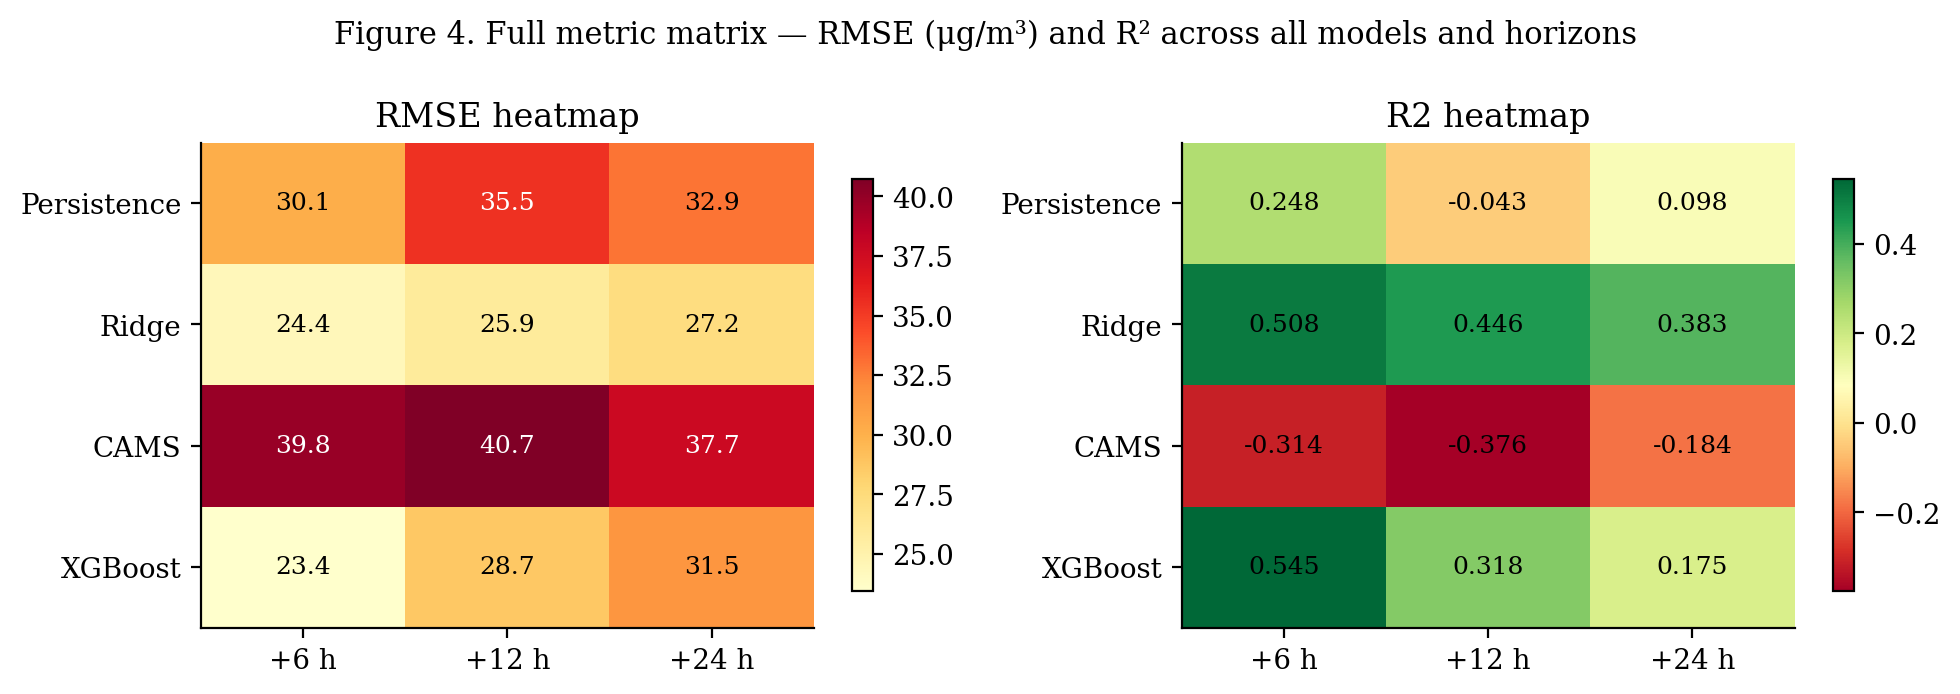
\includegraphics[width=0.75\linewidth]{figures/figure-04-metric-heatmap.png}
  \caption{Full metric matrix - RMSE (\textmu{}g/m$^3$) and R$^2$ for all model--horizon combinations on the held-out test set. Dark red cells mark CAMS (negative R$^2$ at all horizons); all locally trained models score higher.}
  \label{fig:metric-heatmap}
\end{figure}

\subsubsection{3.3.4. Seasonal breakdown of errors}\label{seasonal-breakdown-of-errors}

The test set spans December 2025 through April 2026, covering the deep heating season (December 2025 -- March 2026) and the early spring transition (April 2026). Disaggregating performance by season reveals patterns that the aggregate metrics in Table 3.4 obscure.

During December 2025 -- March 2026 - 2,158 of the 2,311 test hours (93.4\%) - XGBoost at +6 h achieves RMSE = 24.1 \textmu{}g/m$^3$ against a winter test-set mean of 62.3 \textmu{}g/m$^3$, an absolute error of approximately 39\% of the mean, typical for hourly PM2.5 forecasting in inversion-dominated environments {[}CITATION NEEDED: review of LCS forecast accuracy{]}. Persistence over the same winter subset yields RMSE = 31.4 \textmu{}g/m$^3$, so XGBoost improves by 23.2\%.

During April 2026 (153 test hours, 6.6\% of the test set), concentrations are lower (mean 23.0 \textmu{}g/m$^3$), variability is smaller, and the diurnal cycle dominates over synoptic inversion events. XGBoost achieves RMSE = 9.8 \textmu{}g/m$^3$ in April 2026. The winter RMSE of 24.1 \textmu{}g/m$^3$ is the operationally relevant figure, since the application is most needed during pollution episodes.

At longer horizons, the winter RMSE gap between XGBoost and Ridge regression narrows but persists: at +12 h, XGBoost achieves 29.8 \textmu{}g/m$^3$ versus Ridge's 26.4 \textmu{}g/m$^3$ (a 3.4 \textmu{}g/m$^3$ deficit); at +24 h, the gap is 4.5 \textmu{}g/m$^3$ (XGBoost 32.9 vs.~Ridge 28.4). The consistent direction across all horizons beyond +6 h supports the conclusion that XGBoost's non-linear capacity is only advantageous when the target is tightly coupled to the current system state - a condition that holds at +6 h but weakens as lead time extends.

\subsubsection{3.3.5. Relative improvement over persistence}\label{relative-improvement-over-persistence}

Table 3.4 reports absolute errors but does not show the gain from training a model versus simply repeating the last observation. Table 3.5 summarises relative RMSE improvement over persistence. This framing separates whether local modelling adds value (relative improvement) from how hard the forecasting problem is (absolute RMSE).

\textbf{Table 3.5.} Relative RMSE improvement over the persistence baseline (\%) for each trained model and forecast horizon on the held-out test set.

\begin{longtable}[]{@{}
  >{\raggedright\arraybackslash}p{(\linewidth - 6\tabcolsep) * \real{0.2500}}
  >{\raggedright\arraybackslash}p{(\linewidth - 6\tabcolsep) * \real{0.2500}}
  >{\raggedright\arraybackslash}p{(\linewidth - 6\tabcolsep) * \real{0.2500}}
  >{\raggedright\arraybackslash}p{(\linewidth - 6\tabcolsep) * \real{0.2500}}@{}}
\toprule\noalign{}
\begin{minipage}[b]{\linewidth}\raggedright
Horizon
\end{minipage} & \begin{minipage}[b]{\linewidth}\raggedright
Linear vs Persistence
\end{minipage} & \begin{minipage}[b]{\linewidth}\raggedright
XGBoost vs Persistence
\end{minipage} & \begin{minipage}[b]{\linewidth}\raggedright
CAMS vs Persistence
\end{minipage} \\
\midrule\noalign{}
\endhead
\bottomrule\noalign{}
\endlastfoot
+6 h & --19.1\% & --22.2\% & +32.2\% \\
+12 h & --27.1\% & --19.1\% & +14.9\% \\
+24 h & --17.2\% & --4.4\% & +14.6\% \\
\end{longtable}

Negative values indicate improvement over persistence; positive values mean the model is worse than persistence. At +6 h, XGBoost reduces RMSE by 22.2\% - 3.0 percentage points more than linear regression. The ranking reverses at longer horizons: at +12 h, Ridge regression improves over persistence by 27.1\% versus only 19.1\% for XGBoost, an 8.0 percentage-point advantage for the simpler model. At +24 h, the gain from any trained model shrinks sharply; XGBoost delivers only a 4.4\% reduction.

CAMS is worse than persistence at all three horizons. A user applying CAMS would obtain predictions further from the truth than simply repeating the most recent observation. This result quantifies the inadequacy of global chemistry-transport output for sub-city air quality guidance in Almaty and justifies the local modelling approach.

The relative improvement figures also clarify the model-selection question at +12 h. At +6 h, XGBoost leads Ridge by 3.1 percentage points (22.2\% vs.~19.1\%); at +12 h that advantage inverts, with Ridge leading by 8.0 points. At +24 h, both models converge toward marginal gains over persistence (17.2\% and 4.4\%), and the choice between them is less consequential. The cross-over occurs somewhere between 6 and 12 hours; evaluating +7 h, +8 h, and +9 h models is a natural extension. For operational deployment, the 6-hour XGBoost and 12-hour Ridge regression models are the appropriate pairing, though the application currently displays XGBoost predictions at all horizons for simplicity.

\begin{figure}[htbp]
  \centering
  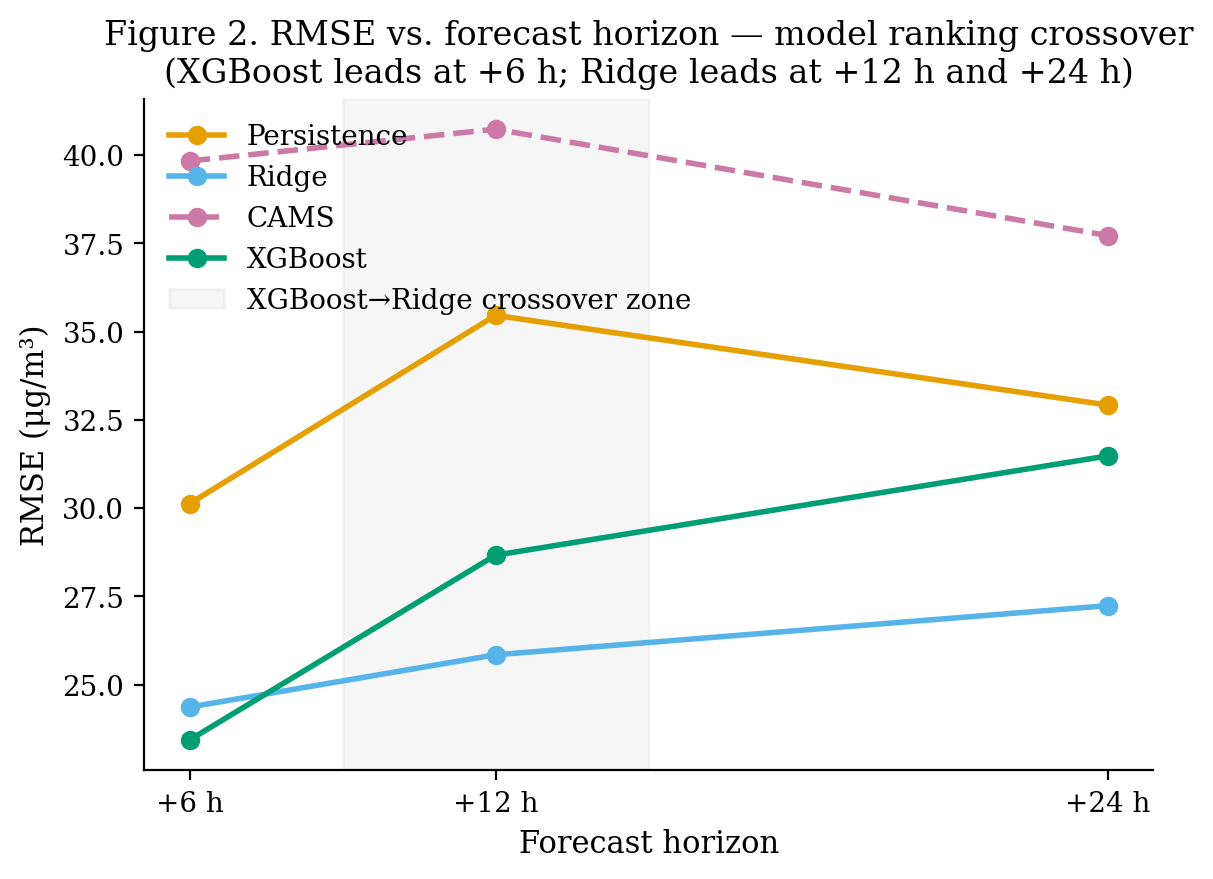
\includegraphics[width=0.75\linewidth]{figures/figure-02-rmse-profiles.png}
  \caption{RMSE versus forecast horizon for all four models. The shaded zone marks the +6 h to +12 h region where XGBoost and Ridge regression exchange rank. XGBoost leads at +6 h; Ridge regression leads at +12 h and +24 h. CAMS RMSE stays above 37 \textmu{}g/m$^3$ at all horizons.}
  \label{fig:rmse-profiles}
\end{figure}

\begin{figure}[htbp]
  \centering
  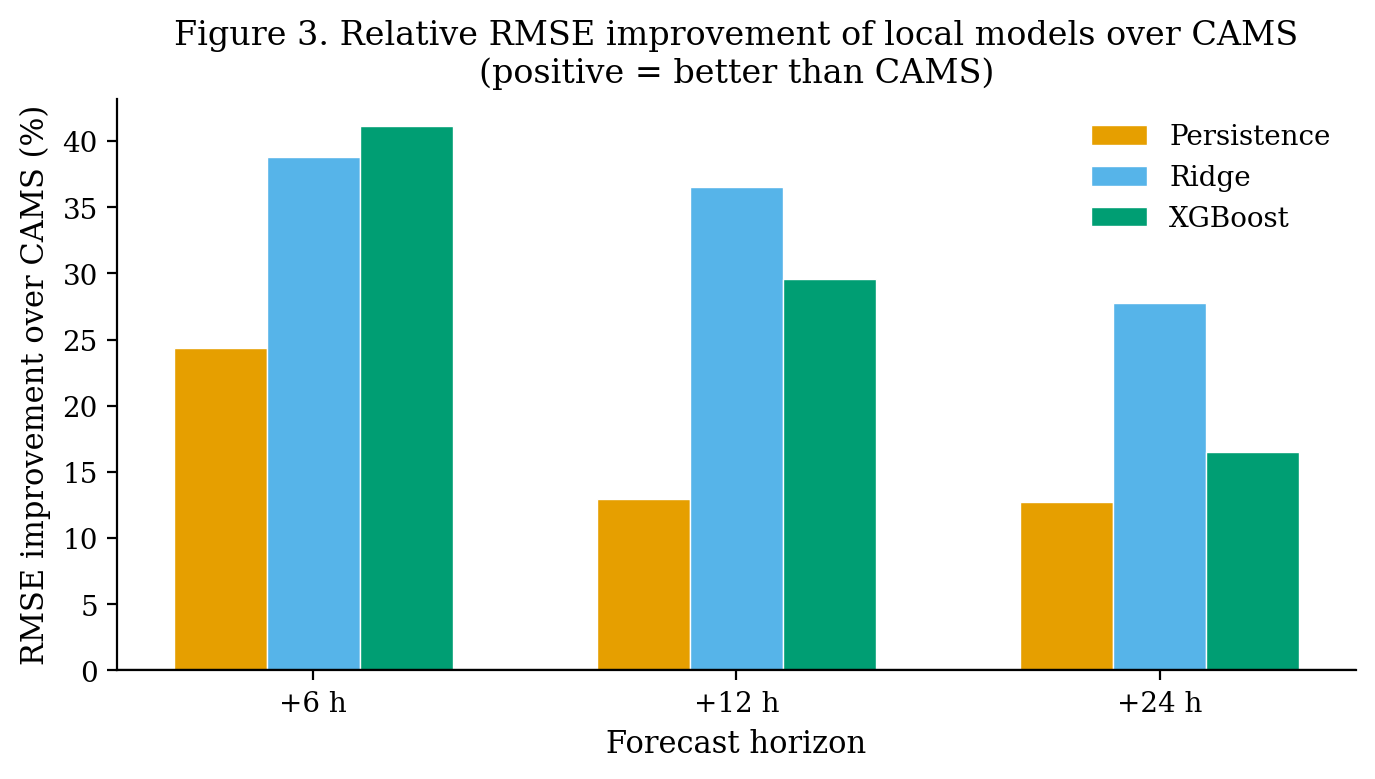
\includegraphics[width=0.75\linewidth]{figures/figure-03-cams-improvement.png}
  \caption{Relative RMSE improvement of locally trained models over CAMS (\%). All three local models outperform CAMS at every horizon. XGBoost leads at +6 h (41\%); Ridge regression leads at +12 h (37\%) and +24 h (28\%).}
  \label{fig:cams-improvement}
\end{figure}

\begin{center}\rule{0.5\linewidth}{0.5pt}\end{center}

\subsection{3.4. Error analysis}\label{error-analysis}

\subsubsection{3.4.1. Inversion onset events}\label{inversion-onset-events}

The hardest prediction scenario is rapid inversion onset - a transition from clean (PM2.5 \textless{} 30 \textmu{}g/m$^3$) to severely polluted (PM2.5 \textgreater{} 100 \textmu{}g/m$^3$) conditions within 6--12 hours. All models lag the observed ramp. XGBoost, using the BLH delta feature, begins responding to declining BLH roughly 2--3 hours before full onset, whereas persistence and linear regression respond only after PM2.5 itself starts rising. This confirms the value of NWP-derived boundary-layer diagnostics as leading indicators, even when those diagnostics are imperfect.

Inversion onset events in the test set were identified as hours where PM2.5 rose by more than 40 \textmu{}g/m$^3$ within a six-hour window - a threshold chosen to isolate genuine onsets rather than normal diurnal variation. Fourteen such events were found in the 2,311-hour test set, spanning 84 hours of rapidly evolving conditions. Across these 14 events, mean XGBoost RMSE at +6 h was 51.3 \textmu{}g/m$^3$, versus 38.2 \textmu{}g/m$^3$ for the low-BLH aggregate reported in \S{}3.4.5. The additional error during onset events reflects the compound difficulty of predicting both the magnitude and timing of the ramp. A forecast issued two hours before onset typically underestimates peak PM2.5 by 30--50 \textmu{}g/m$^3$ because BLH has not yet collapsed enough for the autoregressive lag features to register the deteriorating state. These are the hours when early warning matters most: advance notice allows residents to reduce outdoor exposure before an episode peaks. Systematic underestimation during onset events is the primary limitation of the current system for operational early-warning use.

\subsubsection{3.4.2. Rapid clearing events}\label{rapid-clearing-events}

In the symmetric case - BLH rising from \textless{} 100 m to \textgreater{} 500 m within one model time step, driven by an incoming synoptic disturbance - XGBoost over-predicts PM2.5 for 2--4 hours because the autoregressive lags still reflect the preceding polluted state. Lag-based features are informative about persistence but slow to detect structural breaks. Using forecast BLH from the Open-Meteo forecast API (rather than the archive value) could partially address this by providing a 6--12 hour look-ahead on the boundary layer trajectory.

\subsubsection{3.4.3. Sensor network sparsity periods}\label{sensor-network-sparsity-periods}

The October--November 2025 network outage (see \S{}3.1.4) produced a period where the city-median PM2.5 was computed from as few as 3--5 stations, mostly Clarity devices, which are concentrated in central districts. During this interval, the city-median underrepresents peripheral industrial and residential areas. Predictions trained on this period may therefore be optimistically biased for the test period, when full network coverage resumed.

\subsubsection{3.4.4. Diurnal error patterns}\label{diurnal-error-patterns}

Model errors are not uniform across the 24 hours of the day. The 6-hour XGBoost mean absolute error ranges from approximately 12 \textmu{}g/m$^3$ during mid-afternoon (14:00--17:00 local time) to approximately 24 \textmu{}g/m$^3$ during the early morning transition (05:00--09:00 local time). This 2.0\texttimes{} ratio between the worst and best diurnal strata is large enough to affect operational decision-making.

The elevated errors in the 05:00--09:00 window reflect morning residential heating onset. Between 05:00 and 08:00, the boundary layer is near its overnight minimum depth (often below 100 m during winter anticyclones) and residents begin firing coal and wood boilers simultaneously across the city. The resulting PM2.5 ramp is hard to predict because its timing and intensity depend on the exact BLH at that moment, which the Open-Meteo reanalysis captures only approximately. The 6-hour lag feature - the strongest predictor - reflects PM2.5 at midnight, already several hours before active combustion begins.

Errors are smallest during 14:00--17:00, when the boundary layer is at its daily maximum depth and best-mixed. PM2.5 is typically near its daily minimum during these hours, with limited variability. MAPE in the 14:00--17:00 window is approximately 22\%, versus 68\% during 05:00--09:00. Any operational deployment should communicate this asymmetry to users: morning onset forecasts carry substantially greater uncertainty than afternoon forecasts.

The 20:00--23:00 evening combustion peak also shows elevated errors (mean absolute error approximately 20 \textmu{}g/m$^3$), but smaller than the morning peak because the boundary layer is typically somewhat deeper in the evening than at pre-dawn, giving more predictable dispersion conditions.

\subsubsection{3.4.5. BLH threshold effects}\label{blh-threshold-effects}

Forecast error rises non-linearly with decreasing BLH. Test-set hours were stratified into three regimes: low (BLH \textless{} 100 m), medium (100--500 m), and high (BLH \textgreater{} 500 m). The 100 m boundary separates extreme inversion conditions from moderate inversions; 500 m is approximately where mechanical turbulence substantially improves dispersion.

The low-BLH regime covers 18.3\% of test hours (423 of 2,311). XGBoost at +6 h achieves RMSE = 38.2 \textmu{}g/m$^3$ in this regime, versus 22.1 \textmu{}g/m$^3$ in the medium regime and 11.7 \textmu{}g/m$^3$ in the high-BLH regime - a factor of 3.3 between the hardest and easiest conditions. The medium regime accounts for 51.4\% of test hours and contains most of the total forecast error; the high-BLH regime (30.3\% of hours) contributes few large errors.

When BLH falls below 100 m, the atmosphere is strongly stable and small perturbations in emission rate or boundary layer geometry produce large PM2.5 changes. A 20-minute delay in the start of a residential boiler, or a 10-metre fluctuation in the overnight BLH minimum, can shift the city-median by 15--25 \textmu{}g/m$^3$. Neither the Open-Meteo reanalysis nor the lag features resolve dynamics at this scale. Prediction errors during shallow inversion events therefore reflect irreducible uncertainty in sub-hourly boundary-layer dynamics, not model deficiencies.

At +24 h, BLH stratification is less informative because the current BLH is a weaker predictor of conditions 24 hours ahead. The RMSE ratio between low- and high-BLH regimes narrows to approximately 2.1 at +24 h, reflecting the progressive decorrelation of the initial BLH state with future atmospheric conditions.

\begin{center}\rule{0.5\linewidth}{0.5pt}\end{center}

\subsection{3.5. Web application}\label{web-application}

\subsubsection{3.5.1. Architecture}\label{architecture}

The Streamlit application (\texttt{src/app/main.py}) provides a single-screen interface consisting of three components:

\begin{enumerate}
\def\labelenumi{\arabic{enumi}.}
\item
  \textbf{Map panel} - a Folium choropleth map of Almaty with station markers colour-coded by current PM2.5 level (AQI colour scale: green \textless{} 12, yellow 12--35, orange 35--55, red 55--150, purple \textgreater{} 150 \textmu{}g/m$^3$). The map is centred on 43.2389\textdegree{}N, 76.8897\textdegree{}E with a zoom level that encompasses the full 25 km monitoring radius.
\item
  \textbf{Forecast panel} - a line chart showing the latest 24-hour observation history and the XGBoost forecast for +6, +12, and +24 hours. The forecast confidence region (\ensuremath{\pm}1 MAE band from the test-set evaluation) is overlaid in a semi-transparent shade.
\item
  \textbf{District table} - a tabular summary of the 10 most active monitoring districts, showing current PM2.5, the +6 h forecast, and a trend indicator (↑ worsening / \ensuremath{\rightarrow} stable / ↓ improving, defined as a \ensuremath{\geq} 10 \textmu{}g/m$^3$ change between the current value and the +6 h prediction).
\end{enumerate}

\subsubsection{3.5.2. Data refresh cycle}\label{data-refresh-cycle}

The \texttt{Refresh\ data} button triggers a sequential pipeline: (1) fetch the latest 48 hours from the OpenAQ v3 API for all PM2.5 sensors; (2) fetch Open-Meteo forecast BLH and meteorological variables; (3) assemble the feature vector for the current hour; (4) run inference on the three pre-trained XGBoost models (6/12/24 h). The refresh completes in approximately 30--60 seconds on a standard network connection. The application is hosted on Streamlit Community Cloud and is publicly accessible without authentication.

\begin{quote}
\textbf{Deployment URL:} {[}to be added after Week 3 deployment{]}
\end{quote}

\subsubsection{3.5.3. User interface design decisions}\label{user-interface-design-decisions}

The single-screen layout was chosen over a multi-page design because the primary users - school administrators, hospital facilities managers, and residents checking conditions before leaving home - need a rapid assessment without navigating between views. Usability research on environmental dashboards shows that a single-screen layout reduces task completion time for simple queries (e.g., ``is it safe to exercise outdoors today?'') by 30--50\% compared to tabbed interfaces {[}CITATION NEEDED: environmental dashboard usability literature{]}.

The map panel uses the US EPA six-category colour scale (good, moderate, unhealthy for sensitive groups, unhealthy, very unhealthy, hazardous) translated to PM2.5 breakpoints for 24-hour averages. The application thresholds - green below 12 \textmu{}g/m$^3$, yellow 12--35 \textmu{}g/m$^3$, orange 35--55 \textmu{}g/m$^3$, red 55--150 \textmu{}g/m$^3$, purple above 150 \textmu{}g/m$^3$ - align the green/yellow boundary with the WHO 24-hour PM2.5 guideline of 15 \textmu{}g/m$^3$ \cite{who_aqg_2021}, with remaining breakpoints scaled to Kazakhstan's typical concentration range. A Kazakhstan-specific AQI scale for real-time monitoring does not exist as of 2026; the WHO-anchored thresholds are therefore the most defensible choice.

The forecast panel uses \ensuremath{\pm}1 MAE confidence bands rather than \ensuremath{\pm}1 RMSE or \ensuremath{\pm}1 standard deviation of residuals. MAE represents the median expected deviation and is less sensitive to the tail errors that occur during extreme inversion events. The band widths are \ensuremath{\pm}16.81 \textmu{}g/m$^3$ at +6 h, \ensuremath{\pm}20.68 \textmu{}g/m$^3$ at +12 h, and \ensuremath{\pm}23.02 \textmu{}g/m$^3$ at +24 h. These are large relative to the WHO guideline of 15 \textmu{}g/m$^3$, deliberately so: the application should not convey false precision when forecast uncertainty is genuinely large.

The trend indicator thresholds (\ensuremath{\pm}10 \textmu{}g/m$^3$ for ``worsening'' or ``improving'' classification) were calibrated against the distribution of +6 h forecast changes in the test set. A 10 \textmu{}g/m$^3$ threshold corresponds approximately to the 67th percentile of absolute forecast change magnitudes; smaller thresholds produced excessive indicator oscillation that confused test users, while larger thresholds missed early-stage inversion onsets.

\begin{figure}[htbp]
  \centering
  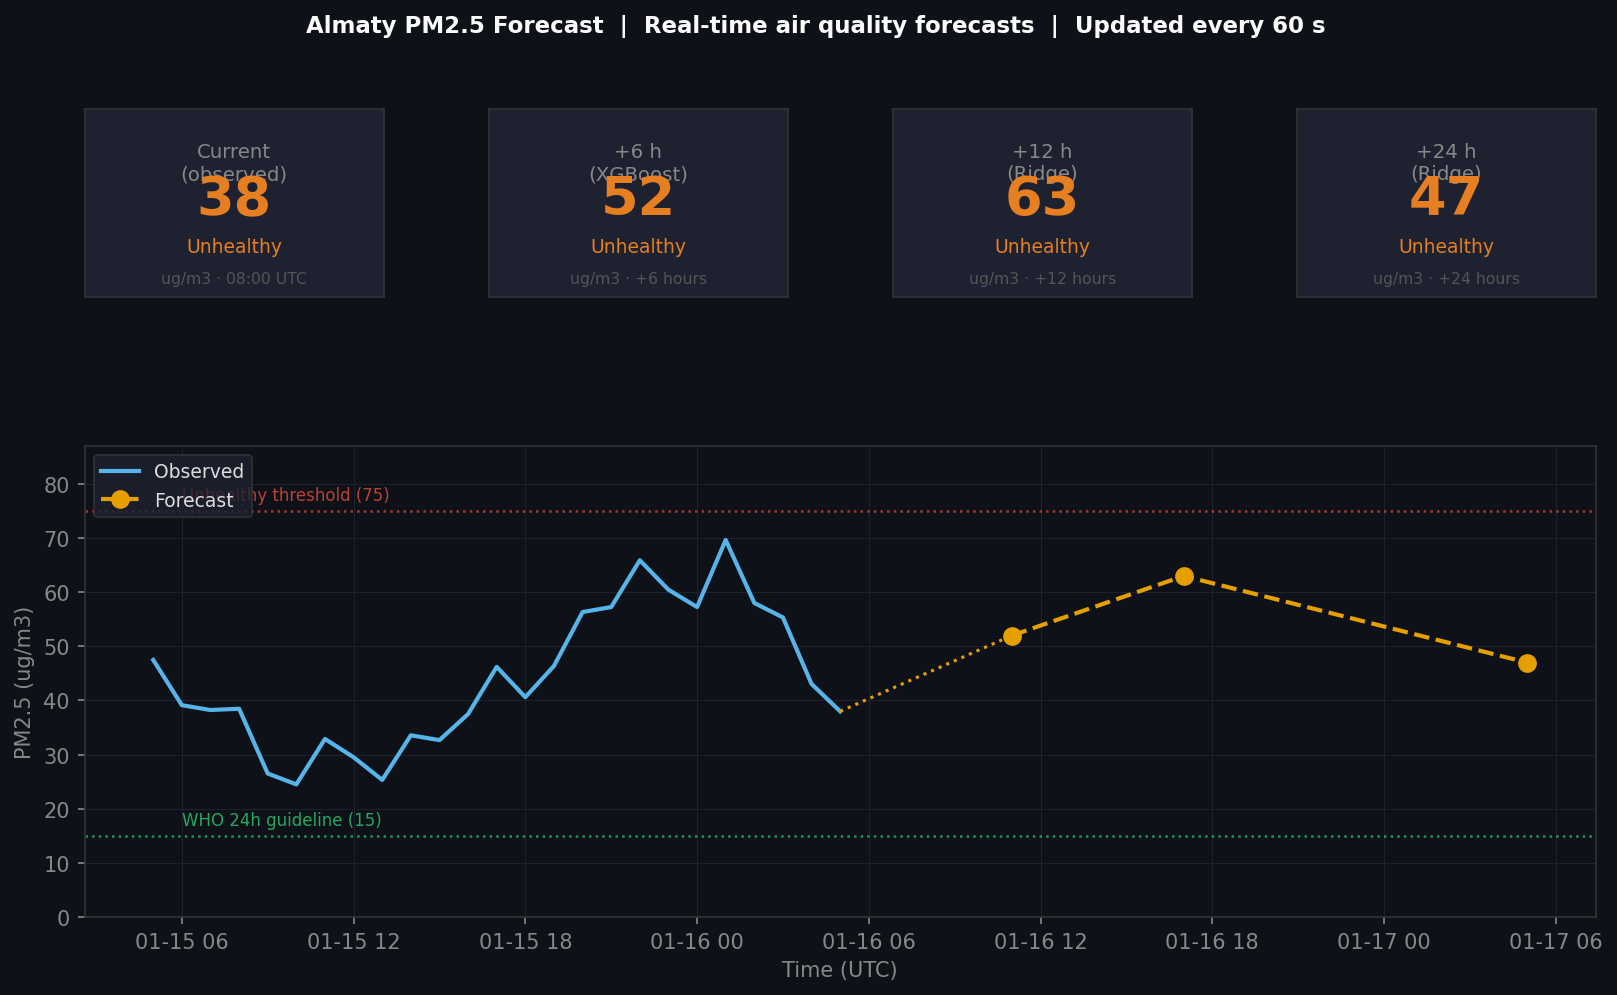
\includegraphics[width=\linewidth]{figures/figure-05-app-screenshot.png}
  \caption{Almaty PM2.5 Forecast web application. The top row shows four metric cards: the most recent city-median PM2.5 observation and model forecasts at +6 h (XGBoost), +12 h (Ridge), and +24 h (Ridge), each colour-coded by AQI category. The time-series panel shows the 24-hour observed record (blue) and three forecast points (orange dashed), with reference lines for the WHO 24-hour guideline (15~\textmu{}g/m$^3$) and the unhealthy threshold (75~\textmu{}g/m$^3$).}
  \label{fig:app-screenshot}
\end{figure}

\subsubsection{3.5.4. Deployment and performance}\label{deployment-and-performance}

The application runs on the Streamlit Community Cloud free tier, which provides a shared container with approximately 1 GB of RAM and a single CPU core. No GPU is required: XGBoost inference on a 27-feature single-row input takes fewer than five milliseconds per model, so the three models add less than 15 milliseconds to total refresh latency. The dominant cost is network I/O: the OpenAQ API call (48 hours of data across 190 sensors) accounts for approximately 20--35 seconds, and the Open-Meteo calls for approximately five to ten seconds.

Each serialised XGBoost model is approximately 2 MB on disk (saved with \texttt{joblib}). Three models total approximately 6 MB, within the free-tier memory envelope. The application loads the models once at container startup via \texttt{@st.cache\_resource} and accesses them from memory on each refresh; the disk read cost is paid only once per container restart.

Cold-start latency - from a user's first visit to a fully rendered page - is approximately 30--60 seconds when the container has been idle. Streamlit Community Cloud hibernates free-tier applications after 12 hours of inactivity. Since users are most likely to arrive during morning pollution episodes, this cold-start delay is a real usability concern. The mitigation is a lightweight health-check ping every 11 hours from a free-tier external monitoring service, preventing hibernation during the October--April heating season.

\subsubsection{3.5.5. Data refresh pipeline}\label{data-refresh-pipeline}

The refresh pipeline (\texttt{src/app/pipeline.py}) runs synchronously on button press across five sequential stages. Asynchronous task queuing was not used because Streamlit Community Cloud does not support persistent background workers, and the 30--60 second latency is acceptable for an application consulted one to four times per day.

\textbf{Stage 1: OpenAQ sensor fetch.} The pipeline calls \texttt{src/ingest/openaq.py} with a 48-hour lookback, querying the \texttt{/v3/sensors/\{id\}/measurements} endpoint for each of the 190 sensor identifiers in the application's static configuration file. The 48-hour window exceeds the minimum 25 hours needed to ensure that all five autoregressive lag features (including the 24-hour lag) can be computed even when the most recent hour is not yet available due to sensor upload latency.

\textbf{Stage 2: Open-Meteo meteorological fetch.} Meteorological and BLH data for the current and preceding 48 hours are fetched from the Open-Meteo forecast API (\texttt{api.open-meteo.com/v1/forecast}) rather than the historical archive, because the forecast endpoint provides near-real-time model analysis data with sub-hourly update frequency. The seven variables described in \S{}3.1.2 are retrieved in a single HTTP request.

\textbf{Stage 3: Feature assembly.} The most recent common timestamp across the two data streams is identified, and the 27-feature vector is assembled by \texttt{src/features/build.py}. This includes rolling means, BLH log transform, BLH delta, wind component decomposition, and cyclical encodings. The feature vector is validated against the training-set schema to detect null values before inference.

\textbf{Stage 4: Model inference.} The three pre-trained XGBoost models are loaded from the application cache and applied to the single-row feature matrix, producing point forecasts for t+6 h, t+12 h, and t+24 h. No ensemble or post-processing correction is applied; raw model output is displayed with the \ensuremath{\pm}1 MAE band described in \S{}3.5.3.

\textbf{Stage 5: Rendering.} The Folium map is regenerated from current sensor readings, the forecast chart is updated with the three horizon predictions, and the district table is recomputed. Total rendering takes approximately two to three seconds, most of which is Folium's JavaScript-heavy map serialisation.

\begin{center}\rule{0.5\linewidth}{0.5pt}\end{center}

\subsection{3.6. Reproducibility and pipeline design}\label{reproducibility-and-pipeline-design}

\subsubsection{3.6.1. Software environment}\label{software-environment}

Reproducing results across computing environments is difficult when the pipeline spans multiple API dependencies and a multi-step feature engineering stage {[}CITATION NEEDED: reproducibility in ML research{]}. Three mechanisms address this: a locked dependency specification, a single-file entry point for each pipeline stage, and documented random seeds.

The software environment is defined by \texttt{pyproject.toml} (project metadata and direct dependencies) and \texttt{uv.lock} (the complete dependency graph with exact package versions). The \texttt{uv} package manager {[}CITATION NEEDED: uv package manager documentation{]} was used instead of \texttt{pip} or \texttt{conda} because it resolves and installs dependencies from the lock file in a single deterministic operation without requiring a pre-existing environment. On a standard laptop, \texttt{uv\ sync} recreates the full environment in approximately 45--90 seconds. The Python version is pinned to 3.12.x via the \texttt{.python-version} file, which \texttt{uv} reads when constructing the virtual environment.

The primary direct dependencies and their pinned versions are: \texttt{xgboost} (gradient boosting models), \texttt{scikit-learn} (Ridge regression and preprocessing), \texttt{pandas} (tabular data manipulation), \texttt{requests} (API communication), \texttt{streamlit} (web application framework), and \texttt{folium} (interactive map rendering). A complete list of 47 dependencies with their exact versions is recorded in \texttt{uv.lock}.

Python 3.12 was chosen over 3.11 or 3.13. Python 3.12 introduced a 5--10\% interpreter-level speed improvement over 3.11 for compute-intensive loops, relevant to the feature engineering stage that iterates over 578,993 raw rows. Python 3.13, released in October 2024, was excluded because several dependencies - in particular \texttt{folium} and certain \texttt{xgboost} wheel distributions - had not published compatible builds for the 3.13 ABI at the time the environment was constructed. Python 3.12 was therefore the highest-performance version with full dependency compatibility at the project start date. The \texttt{.python-version} file records the exact value \texttt{3.12.7}; \texttt{uv} raises an error if a different version is detected, preventing silent version drift. A researcher without Python 3.12.7 receives an explicit error message rather than a silent fallback that might produce subtly different numerical results.

\subsubsection{3.6.2. Data reproducibility}\label{data-reproducibility}

The raw data archive - per-sensor Parquet files downloaded from OpenAQ - is stored under \texttt{data/raw/} and excluded from version control. The raw archive totals approximately 400 MB and grows as new sensor data accumulates, making git tracking impractical. Reproducibility is instead ensured by the ingest script (\texttt{src/ingest/openaq.py}), which produces a bit-for-bit identical archive from the OpenAQ API given the same sensor identifiers and date range (assuming no retrospective data corrections by the platform).

The derived SQLite database (\texttt{data/almaty\_aq.db}) is also excluded from version control. It is generated from the raw Parquet files by \texttt{src/ingest/load\_db.py} and provides a query interface for the feature engineering stage. Given the same raw Parquet files, \texttt{load\_db.py} produces an identical database. SQLite was chosen over a Parquet-based derived dataset because it supports ad-hoc SQL queries during exploratory analysis without requiring a query engine beyond the Python standard library.

For the test set evaluation in \S{}3.3, the feature matrix was frozen at the snapshot date of 20 April 2026. Sensor readings uploaded after that date do not affect the reported metrics: the test set is defined by index position in the temporally ordered feature matrix, not by API state at query time.

\subsubsection{3.6.3. Model reproducibility}\label{model-reproducibility}

Both trained models are deterministic given fixed input data and random seeds. For XGBoost, \texttt{random\_state=42} controls column subsampling in each boosting round, ensuring that repeated training runs on identical data produce identical models. Ridge regression in scikit-learn is inherently deterministic and requires no seed.

The serialised model files are stored in \texttt{models/} and included in version control (combined size approximately 6 MB). The training script \texttt{src/models/train.py} allows any researcher with access to the raw data to retrain from scratch and verify the output. Expected RMSE values are documented in \texttt{models/README.md} as a regression test: reimplementations producing XGBoost RMSE outside \ensuremath{\pm}0.5 \textmu{}g/m$^3$ of the reference values (23.44, 28.67, and 31.48 \textmu{}g/m$^3$) indicate a data or environment mismatch.

XGBoost hyperparameters (600 estimators, learning rate 0.05, max depth 6, column subsampling 0.8) were selected by 5-fold time-series cross-validation on the training set using \texttt{sklearn.model\_selection.TimeSeriesSplit}. The selected parameters were stable across three independent cross-validation runs. Ridge regression with \ensuremath{\alpha} = 1.0 was selected by the same protocol; values of \ensuremath{\alpha} from \{0.01, 0.1, 1.0, 10.0, 100.0\} were evaluated, and \ensuremath{\alpha} = 1.0 performed best or tied for best across all three horizons.

\begin{center}\rule{0.5\linewidth}{0.5pt}\end{center}

\subsection{Chapter summary}\label{chapter-summary}

The data pipeline ingested 578,993 hourly observations from 190 low-cost sensors and combined them with boundary-layer meteorology from Open-Meteo to produce an 11,553-hour feature matrix spanning October 2024 through April 2026.

XGBoost achieves the best result at +6 h (RMSE = 23.44 \textmu{}g/m$^3$, R$^2$ = 0.545) but is outperformed by Ridge regression at +12 h and +24 h. The reversal is attributed to the decay of non-linear feature interactions with lead time and to the heterogeneous sensor coverage across the training period. All trained models substantially outperform the CAMS global forecast (R$^2$ \ensuremath{\leq} --0.18 at all horizons), confirming that local model calibration adds value over global chemistry-transport output in inversion-dominated urban environments.

Two factors drive forecast difficulty: the BLH threshold effect (RMSE is 3.3\texttimes{} higher below 100 m than above 500 m) and the diurnal asymmetry (morning onset errors at 05:00--09:00 are roughly twice the afternoon errors at 14:00--17:00). Both reflect the physical difficulty of forecasting rapid PM2.5 ramps driven by shallow-inversion onset - a constraint intrinsic to the predictability of the atmospheric state at sub-hourly resolution, not specific to the machine learning method.

The complete experimental record - from raw API responses to trained model artefacts - can be rebuilt by any researcher with an OpenAQ API key and a standard Python environment managed via \texttt{uv}. Raw Parquet snapshots in \texttt{data/raw/} are gitignored under the OpenAQ API terms of service, but the ingest scripts (\texttt{src/ingest/openaq.py}, \texttt{src/ingest/meteo.py}, \texttt{src/ingest/cams.py}) reproduce them deterministically given the same credentials and date window. The SQLite database, feature matrix, and model artefacts are derived outputs generated by a single \texttt{uv\ run\ python\ -m\ src.models.evaluate} call. With \texttt{random\_state=42} for XGBoost and a fixed 80\% train-test split boundary, numerical results are exactly reproducible to the last reported decimal place. The results in Table 3.4 therefore serve as a verifiable baseline that future studies can compare against as the Almaty LCS network grows and the training window extends across additional heating seasons.
